\begin{exercise}{2.2}\label{ex:bezier_spline}
    Implement the de Casteljau algorithm for a planar Bézier curve of arbitrary degree $d$ over a general interval $[a, b]$.
    Use the routine to make a program to plot the quadratic spline curve $\mathbf{s} : [0, 2] \to \mathbb{R}$, with pieces
    \begin{align*}
        \mathbf{p}(t) &= \sum_{i=0}^{2} \mathbf{c}_i B_{i}^2(t), & 0 \leq t \leq 1, \\
        \mathbf{q}(t) &= \sum_{i=0}^{2} \mathbf{d}_i B_{i}^2(t - 1), & 1 < t \leq 2,
    \end{align*}
    where $\mathbf{c}_0 = (-1, 1)$, $\mathbf{c}_1 = (-1, 0)$, $\mathbf{c}_2 = (0, 0)$, and $\mathbf{d}_0 = (0, 0)$, $\mathbf{d}_1 = (1, 0)$, $\mathbf{d}_2 = (2, 1)$.
\end{exercise}

\begin{solution}{2.2}
    The de Casteljau algorithm is implemented in \verb|spline_cj.py|\footnote{\href{https://github.com/augustfe/MAT4170/blob/main/doc/2_splines_in_bb/spline_cj.py}{Available here.}}, and is practically identical to the one implemented in the previous section, due to the vectorization possibilities in \verb|JAX|.
    The resulting figure is shown in \cref{fig:bezier_spline}.
    \begin{figure}[ht]
        \centering
        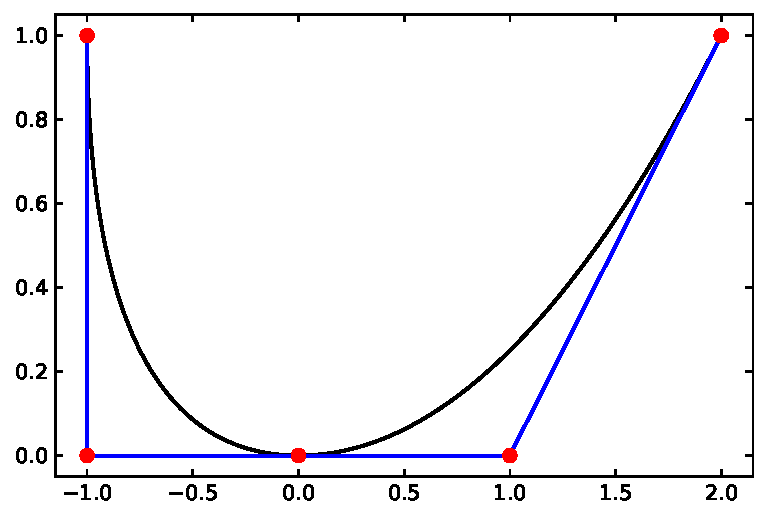
\includegraphics[width=0.7\textwidth]{../doc/2_splines_in_bb/bezier_casteljau.pdf}
        \caption{The quadratic spline curve $\mathbf{s} : [0, 2] \to \mathbb{R}$, with pieces $\mathbf{p}(t)$ and $\mathbf{q}(t)$.\label{fig:bezier_spline}}
    \end{figure}
\end{solution}

\begin{exercise}{2.3}
    What is the order of continuity of $\mathbf{s}$ in \cref{ex:bezier_spline} at the breakpoint $t = 1$?
\end{exercise}

\begin{solution}{2.3}
    We clearly have $C^0$ continuity at the breakpoint $t = 1$, as
    \begin{equation*}
        \mathbf{c}_2 = (0, 0) = \mathbf{d}_0.
    \end{equation*}
    For $C^1$ continuity, we must have
    \begin{align*}
        \frac{\mathbf{c}_2 - \mathbf{c}_1}{1 - 0} &= \frac{\mathbf{d}_1 - \mathbf{d}_0}{2 - 1} \\
        (0, 0) - (-1, 0) &= (1, 0) - (0, 0),
    \end{align*}
    which also holds.
    Finally for $C^2$ continuity, we must have
    \begin{align*}
        \frac{\mathbf{c}_2 - 2 \mathbf{c}_1 + \mathbf{c}_0}{1^2} &\stackrel{?}{=} \frac{\mathbf{d}_2 - 2 \mathbf{d}_1 + \mathbf{d}_0}{1^2} \\
        (0, 0) - 2(-1, 0) + (-1, 1) = (1, 1) &\neq (0, 1) = (2, 1) - 2(1, 0) + (0, 0),
    \end{align*}
    which it seems like we do not have.
    Thus, the order of continuity of $\mathbf{s}$ at the breakpoint $t = 1$ is $C^1$.
\end{solution}

\begin{exercise}{3.1}
    Suppose that $x_0, x_1, x_2$ are distinct, and let $f_i = f(x_i)$, $i = 0, 1, 2$, for some function $f$.
    Show by direct calculation that the recursive formula
    \begin{equation*}
        [x_0, x_1, x_2]f =
        \frac{
            \frac{f_2 - f_1}{x_2 - x_1}
            - \frac{f_1 - f_0}{x_1 - x_0}
        }{x_2 - x_0}
    \end{equation*}
    can be expressed as
    \begin{equation*}
        [x_0, x_1, x_2]f = \sum_{i=0}^{2} \frac{f_i}{\prod_{j \neq i} (x_i - x_j)}.
    \end{equation*}
\end{exercise}

\begin{solution}{3.1}
    We have
    \begin{align*}
        [x_0, x_1, x_2]f
        &= \frac{
            \frac{f_2 - f_1}{x_2 - x_1}
            - \frac{f_1 - f_0}{x_1 - x_0}
        }{x_2 - x_0}
    \end{align*}
    where we begin by expanding the top fractions.
    \begin{align}
        \frac{f_2 - f_1}{x_2 - x_1} - \frac{f_1 - f_0}{x_1 - x_0}
        &= \frac{f_2}{x_2 - x_1} - f_1 \left( \frac{1}{x_2 - x_1} + \frac{1}{x_1 - x_0} \right) + \frac{f_0}{x_1 - x_0} \nonumber \\
        &= \frac{f_2}{x_2 - x_1} - f_1 \frac{x_1 - x_0 + x_2 - x_1}{(x_2 - x_1)(x_1 - x_0)} + \frac{f_0}{x_1 - x_0} \nonumber \\
        &= \frac{f_2}{x_2 - x_1} - f_1 \frac{x_2 - x_0}{(x_2 - x_1)(x_1 - x_0)} + \frac{f_0}{x_1 - x_0} \nonumber \\
        &= \frac{f_2}{x_2 - x_1} + \frac{f_1(x_2 - x_0)}{(x_1 - x_2)(x_1 - x_0)} + \frac{f_0}{x_1 - x_0} \label{eq:top_fraction}
    \end{align}
    Dividing~\eqref{eq:top_fraction} by $x_2 - x_0$ gives
    \begin{align*}
        [x_0, x_1, x_2]f
        &= \frac{
            \frac{f_2 - f_1}{x_2 - x_1}
            - \frac{f_1 - f_0}{x_1 - x_0}
        }{x_2 - x_0} \\
        &= \frac{f_2}{(x_2 - x_1)(x_2 - x_0)}
        + \frac{f_1}{(x_1 - x_2)(x_1 - x_0)}
        + \frac{f_0}{(x_1 - x_0)(x_2 - x_0)} \\
        &= \frac{f_2}{(x_2 - x_1)(x_2 - x_0)}
        + \frac{f_1}{(x_1 - x_2)(x_1 - x_0)}
        + \frac{f_0}{(x_0 - x_1)(x_0 - x_2)} \\
        &= \sum_{i=0}^{2} \frac{f_i}{\prod_{j \neq i} (x_i - x_j)},
    \end{align*}
    as desired.
\end{solution}

\begin{exercise}{3.3}
    Show that if $f(x) = 1/x$ and that $x_0, x_1, \ldots, x_k \neq 0$ then
    \begin{equation*}
        [x_0, \ldots, x_k]f = (-1)^k \frac{1}{x_0 x_1 \cdots x_k}.
    \end{equation*}
\end{exercise}

\begin{solution}{3.3}
    In the base case we have simply
    \begin{equation*}
        [x_0]f = \frac{1}{x_0} = (-1)^0 \frac{1}{x_0}.
    \end{equation*}
    In the case of $x_0 = x_1 = \cdots = x_k$ we have
    \begin{equation*}
        [\underbrace{x_0, x_0, \ldots, x_0}_{k+1}]f = \frac{f^{(k)}(x_0)}{k!} = (-1)^k \frac{1}{x_0^{k+1}} \frac{k!}{k!} = (-1)^k \frac{1}{x_0 x_1 \cdots x_k},
    \end{equation*}
    so mulitplicities are handled correctly.
    For two distinct points $x_0, x_1$ we have
    \begin{equation*}
        [x_0, x_1]f = \frac{f_1 - f_0}{x_1 - x_0} = \frac{1/x_1 - 1/x_0}{x_1 - x_0} = \frac{x_0 - x_1}{x_0 x_1 (x_1 - x_0)} = (-1)^1 \frac{1}{x_0 x_1},
    \end{equation*}
    so the formula holds for $k = 1$.
    Assume that the formula holds for $k = n$, and consider $k = n + 1$.
    We have
    \begin{align*}
        [x_0, \ldots, x_{n+1}]f
        &= \frac{[x_1, \ldots, x_{n+1}]f - [x_0, \ldots, x_{n}]f}{x_{n+1} - x_0} \\
        &= \frac{(-1)^n \frac{1}{x_1 \cdots x_{n+1}} - (-1)^n \frac{1}{x_0 \cdots x_n}}{x_{n+1} - x_0} \\
        &= (-1)^n \frac{
            \frac{1}{x_{n+1}} - \frac{1}{x_0}
        }{
            (x_{n+1} - x_0) x_1 \cdots x_n
        } \\
        &= (-1)^n  \frac{
            \frac{x_0 - x_{n+1}}{x_0 x_{n+1}}
        }{
            (x_{n+1} - x_0) x_1 \cdots x_n
        } \\
        &= (-1)^{n+1}\frac{
            x_{n+1} - x_0
        }{
            (x_{n+1} - x_0) x_0 x_1 \cdots x_n x_{n+1}
        } \\
        &= (-1)^{n+1}\frac{1}{x_0 x_1 \cdots x_{n+1}},
    \end{align*}
    proving the formula by induction.
\end{solution}

\begin{exercise}{3.5}
    Use the recursion formula (Theorem~3.4) to show that
    \begin{enumerate}[
    label=\alph*) % chktex 9 % tex-fmt: skip
            ] % chktex 10
        \item $B[0, 0, 0, 1](x) = (1 - x)^2 B[0, 1](x)$,
        \item $B[0, 0, 1, 2](x) = x(2 - 3x/2)B[0, 1](x) + \frac{1}{2}(2 - x)^2B[1, 2](x)$,
        \item $B[0, 1, 1, 2](x) = x^2B[0, 1](x) + (2 - x)^2B[1, 2](x)$.
    \end{enumerate}
\end{exercise}

\begin{solution}{3.5}
    The recursion formula states that for $d \geq 1$,
    \begin{equation*}
        B_{i, d}(x)
        = \frac{x - t_i}{t_{i+d} - t_i} B_{i, d-1}(x)
        + \frac{t_{i+d+1} - x}{t_{i+d+1} - t_{i+1}} B_{i+1, d-1}(x).
    \end{equation*}
    I'm not entirely sure which knots the $B$-splines are defined on, however I guess the exercise is to relate these ones to the cardinal $B$-splines.

    \begin{enumerate}[
    label=\alph*) % chktex 9 % tex-fmt: skip
            ] % chktex 10
        \item In this case we have $t_i = t_d$, meaning that the first term in the recursion formula is zero.
            We then have
            \begin{align*}
                B[0, 0, 0, 1](x)
                = 0 + \frac{1 - x}{1 - 0} B[0, 0, 1](x).
            \end{align*}
            Recursing on $B[0, 0, 1](x)$, again the first term is zero, so we have
            \begin{equation*}
                (1 - x)B[0, 0, 1](x)
                = (1-x) \frac{1 - x}{1 - 0} B[0, 1](x)
                = (1 - x)^2 B[0, 1](x).
            \end{equation*}

        \item Next, we have
            \begin{gather*}
                B[0, 0, 1, 2](x)
                = \frac{x - 0}{1 - 0} B[0, 0, 1](x)
                + \frac{2 - x}{2 - 0} B[0, 1, 2](x) \\
                = x (1 - x) B[0, 1](x)
                + \frac{2 - x}{2} \left(
                    x B[0, 1](x)
                    + (2 - x) B[1, 2](x)
                \right) \\
                = x \left( 1 - x + \frac{2 - x}{2} \right) B[0, 1](x)
                + \frac{1}{2}(2 - x)^2 B[1, 2](x) \\
                = x \left( 2 - \frac{3}{2}x \right) B[0, 1](x)
                + \frac{1}{2}(2 - x)^2 B[1, 2](x).
            \end{gather*}

        \item Finally, for the last expression we have
            \begin{equation*}
                B[0, 1, 1, 2](x)
                = \frac{x - 0}{1 - 0} B[0, 1, 1](x)
                + \frac{2 - x}{2 - 1} B[1, 1, 2](x).
            \end{equation*}
            Considering the two terms separately, we have
            \begin{equation*}
                B[0, 1, 1](x)
                = x B[0, 1](x)
            \end{equation*}
            as the second term vanishes, and
            \begin{equation*}
                B[1, 1, 2](x)
                = \frac{2 - x}{2 - 1} B[1, 2](x)
                = (2 -x)^2 B[1, 2](x),
            \end{equation*}
            where the first term vanishes.
            Combining these, we find
            \begin{equation*}
                B[0, 1, 1, 2](x)
                = x^2 B[0, 1](x) + (2 - x)^2 B[1, 2](x),
            \end{equation*}
            as desired.
    \end{enumerate}
\end{solution}

\begin{exercise}{B-splines.}
    What are the smoothness properties of $B[0, 0, 0, 0, 1](x)$ and $B[0, 1, 1, 1, 2](x)$?
\end{exercise}

\begin{solution}{B-splines.}
    The smoothness of a $B$-spline of degree $d$ at a knot with multiplicity $m$ is $C^{d-m}$.
    Denoting $B[0, 0, 0, 0, 1](x)$ as $B^1(x)$, we have that the degree of $B^1$ is $d = 3$.
    $0$ has a multiplicity of four, so the smoothness of $B^1$ at $0$ is $C^{-1}$.
    At $1$, the multiplicity is $1$, so the smoothness is $C^2$.
    Between the knots, the smoothness is $C^\infty$.

    Denoting $B[0, 1, 1, 1, 2](x)$ as $B^2(x)$, we that the degree of $B^2$ is $d = 3$.
    $0$ and $2$ both have a multiplicity of one, so the smoothness is $C^2$ at both points.
    $1$ has a multiplicity of three, so the smoothness at this point is $C^{0}$.
\end{solution}

\begin{exercise}{2.4 (\textit{Optional})}
    The curvature of a parametric curve $\mathbf{r}(t)$ in $\mathbb{R}^2$ can be expressed as
    \begin{equation*}
        \kappa(t) = \frac{\mathbf{r}'(t) \times \mathbf{r}''(t)}{\norm{\mathbf{r}'(t)}^3},
    \end{equation*}
    where $(a_1, a_2) \times (b_1, b_2) := a_1 b_2 - a_2 b_1$.
    What are the curvatures of $\mathbf{p}$ and $\mathbf{q}$ in Exercise~\ref{ex:bezier_spline} at the breakpoint $t = 1$?
    What can you say about the smoothness of $\mathbf{s}$?
\end{exercise}

\begin{solution}{2.4 (\textit{Optional})}
    We firstly begin by tabulating the derivatives of $\mathbf{p}$ and $\mathbf{q}$, based on the general formula
    \begin{equation*}
        p^{(r)}(x) = \frac{d!}{(d - r)!} \frac{1}{h^r} \sum_{i=0}^{d-r} \Delta^r c_{i} B_i^{d-r}(\lambda).
    \end{equation*}
    In both cases here, we have $h = 1$, $d = 2$, and $\lambda = t$ for $\mathbf{p}$ and $\lambda = t - 1$ for $\mathbf{q}$.
    The derivatives for $\mathbf{p}$ are then
    \begin{align*}
        \mathbf{p}'(t) &= 2 \left(\left( \mathbf{c}_1 - \mathbf{c}_0 \right) B_0^1(\lambda) + \left( \mathbf{c}_2 - \mathbf{c}_1 \right) B_1^1(\lambda)\right) &
        \mathbf{p}''(t) &= 2 \left( \mathbf{c}_2 - 2 \mathbf{c}_1 + \mathbf{c}_0 \right) B_0^0(\lambda) \\
        &= 2 \left(\left( \mathbf{c}_1 - \mathbf{c}_0 \right) (1 - t) + \left( \mathbf{c}_2 - \mathbf{c}_1 \right) t\right) &
        &= 2 \left(1, 1\right) \\
        &= 2 \left(
            (\mathbf{c}_2 - 2 \mathbf{c}_1 + \mathbf{c}_0)t + (\mathbf{c}_1 - \mathbf{c}_0)
        \right) &
        &= (2, 2), \\
        &= 2 \left(
            (1, 1)t + (0, -1)
        \right) \\
        &= (2t, 2t - 2),
    \end{align*}
    while we for $\mathbf{q}$ have
    \begin{align*}
        \mathbf{q}'(t) &= 2 \left(\left( \mathbf{d}_1 - \mathbf{d}_0 \right) B_0^1(\lambda) + \left( \mathbf{d}_2 - \mathbf{d}_1 \right) B_1^1(\lambda)\right) &
        \mathbf{q}''(t) &= 2 \left( \mathbf{d}_2 - 2 \mathbf{d}_1 + \mathbf{d}_0 \right) B_0^0(\lambda) \\
        &= 2 \left(\left( \mathbf{d}_1 - \mathbf{d}_0 \right) t + \left( \mathbf{d}_2 - \mathbf{d}_1 \right) (1 - t)\right) &
        &= 2 \left(0, 1\right) \\
        &= 2 \left(
            (-\mathbf{d}_2 + 2 \mathbf{d}_1 - \mathbf{d}_0)t + (\mathbf{d}_2 - \mathbf{d}_1)
        \right) &
        &= (0, 2), \\
        &= 2 \left(
            (0, -1)t + (1, 1)
        \right) \\
        &= (2, - 2t + 2),
    \end{align*}
    where we have used that $B_0^1(1 - t) = t$ and $B_1^1(1 - t) = 1 - t$.
    The curvatures are then
    \begin{align*}
        \kappa_{\mathbf{p}}(t) &= \frac{(2t, 2t - 2) \times (2, 2)}{\sqrt{(2t)^2 + (2t - 2)^2}^3} = \frac{4}{(8t^2 - 8t + 4)^{3/2}}, \\
        \kappa_{\mathbf{q}}(t) &= \frac{(2, -2t + 2) \times (0, 2)}{\sqrt{2^2 + (-2t + 2)^2}^3} = \frac{4}{(4t^2 - 8t + 8)^{3/2}}.
    \end{align*}
    These give, at the breakpoint $t = 1$, the curvatures
    \begin{equation*}
        \kappa_{\mathbf{p}}(1) = \frac{4}{2^3} = \frac{1}{2}
        \quad \text{and} \quad
        \kappa_{\mathbf{q}}(1) = \frac{4}{2^3} = \frac{1}{2}.
    \end{equation*}
    As we see, the curvatures are equal at the breakpoint $t = 1$.
    This means that while we do not have $C^2$ continuity, we have $G^2$ continuity / smoothness.
\end{solution}